\documentclass[conference]{IEEEtran}
% If the IEEEtran.cls has not been installed into the LaTeX system files, 
% manually specify the path to it:
% \documentclass[conference]{../sty/IEEEtran} 

\ifx\pdfoutput\undefined
\usepackage{graphicx}
\else
\usepackage[pdftex]{graphicx}
\fi

\usepackage{helvet}		
\usepackage[T1]{fontenc}		% Selecao de codigos de fonte.
\usepackage[utf8]{inputenc}		% Codificacao do documento (conversão automática dos acentos)
\usepackage{color}				% Controle das cores
\usepackage{microtype} 			% para melhorias de justificação
\usepackage[colorlinks=true, linkcolor=black, citecolor=black, urlcolor=black]{hyperref}
\usepackage{times}

\usepackage{amsmath}

\usepackage{lipsum}				% para geração de dummy text
\usepackage{import}
\usepackage{blindtext}
\usepackage{soul}
\usepackage{lscape}

\usepackage{algpseudocode}
\usepackage{algorithm}
\algnewcommand{\LineComment}[1]{\State \(\triangleright\) #1}
\makeatletter
\renewcommand{\ALG@name}{Algoritmo}
\makeatother

\graphicspath{ {../images/} }

\newcommand{\un}[1]{\;\text{#1}}

\hyphenation{op-tical net-works semi-conduc-tor IEEEtran}

\begin{document}

% paper title
\title{Trabalho Computacional 3 - Teoria da Decisão (ELE088)}

\author{\authorblockN{Daniel Felipe de Almeida Araújo}
\authorblockA{Universidade Federal de Minas Gerais\\
Matrícula: 2023422617}
\and
\authorblockN{Milton Pereira Bravo Neto}
\authorblockA{Universidade Federal de Minas Gerais\\
Matrícula: 2018072549}
\and
\authorblockN{Raphael Henrique Braga Leivas}
\authorblockA{Universidade Federal de Minas Gerais\\
Matrícula: 2020028101}
}

\maketitle

\begin{abstract}
The abstract goes here.
\end{abstract}

\section{Introdução}
% no \PARstart
This demo file is intended to serve as a ``starter file"
for IEEE conference papers produced under \LaTeX\ using IEEEtran.cls version
1.6b and later.

 May all your publication endeavors be successful.

\hfill mds
 
\hfill November 18, 2002

\section{Metodologia}


\subsection{Modelagem do Problema}
Inicialmente podemos ver o trabalho como sendo dois problemas mono-objetivo distintos:

\begin{itemize}
	\item Problema 1: minimização do custo de manutenção total $f_1 (\cdot)$
	\item Problema 2: minimização do custo esperado de falha total $f_2 (\cdot)$
\end{itemize}

\subsubsection{Problema 1}

Temos essencialmente um problema de designação simples. Seja $N$ o número de 
equipamentos e $J$ o número de políticas de manutenção, definimos a variável de decisão $x_{ij}$ 
por

\begin{equation}
	x_{ij}: \un{se o equipamento $i$ executa a manutenção $j$}
\end{equation}

\noindent onde 

\[ x_{ij} \in \{0,1\} \quad , \quad i = \{1, 2, ..., N\}  \quad , \quad j = \{1, 2, ..., J\} \]

Para a função objetivo, seja $c_j$ o custo de executar a manutenção $j$. Note que esse custo 
independe do equipamento $i$ que estamos executando a manutenção. Temos a função objetivo  

\begin{equation}\label{eq:objf1}
	\min f_1 = \sum_{i=1}^{N} \sum_{j=1}^{J} c_j x_{ij}
\end{equation}

\noindent sujeito a 

\begin{equation}\label{eq:restf1}
	\sum_{j=1}^{J} x_{ij} = 1 \quad , \quad \forall i = {1, 2, ..., N}
\end{equation}

A \ref{eq:restf1} indica que todo equipamento executa exatamente uma política de manutenção.
Além disso, note que solução da \ref{eq:objf1} é trivial: basta escolher o plano de 
manutenção com o menor custo para todos os equipamentos.

\subsubsection{Problema 2}

O custo da falha de cada equipamento é dado pelo produto da probabilidade de falha $p_{ij}$ pelo custo da falha do equipamento,
dada por $d_i$. Assim, temos 

\begin{equation}\label{eq:objf2}
	\min f_2 = \sum_{i=1}^{N} \sum_{j=1}^{J} p_{ij} \, d_i \, x_{ij}
\end{equation}

\noindent onde 

\[ x_{ij} \in \{0,1\} \quad , \quad i = \{1, 2, ..., N\}  \quad , \quad j = \{1, 2, ..., J\} \]


\begin{equation}\label{eq:pij}
	p_{ij} = \frac{F_i \left(t_0 + k_j \Delta t \right) - F_i\left(t_0\right) }{1 - F_i\left(t_0\right)}
\end{equation}
\begin{equation}\label{eq:fit}
	F_i(t) = 1 - \exp \left[ - \left( \frac{t}{\eta_i} \right)^{\beta_i} \right]
\end{equation}


\noindent sujeito a 

\begin{equation}\label{eq:restf2}
	\sum_{j=1}^{J} x_{ij} = 1 \quad , \quad \forall i = {1, 2, ..., N}
\end{equation}

Note que na Equação \ref{eq:objf2} temos essencialmente um problema de programação linear inteira.
Assim, é possível usar o método Simplex visto em Pesquisa Operacional para resolver esse problema
com garantia de otimalidade. Usando o Simplex, a solução encontrada foi 

\[ \mathbf{x^{*}}  = \begin{bmatrix} 
	0 & 0 & 1 \\
	0 & 0 & 1 \\
	\vdots & \vdots & \vdots \\
	0 &  0      & 1 
	\end{bmatrix} \quad , \quad f_2\left(\mathbf{x^{*}}\right) = 1048.17  \]

Assim, antes mesmo de começar a implementar o BVNS para resolver os problemas isoladamente, 
já sabemos as soluções ótimas para eles.

\subsubsection{Modelagem Multiobjetivo}

Juntando as modelagens dos problemas mono-objetivos acima, temos 
a modelagem multiobjetivo do problema.

\[  \min f_1 = \sum_{i=1}^{N} \sum_{j=1}^{J} c_j x_{ij} \]

\[  \min f_2 = \sum_{i=1}^{N} \sum_{j=1}^{J} p_{ij} \, d_i \, x_{ij} \]

\[  x_{ij}: \un{se o equipamento $i$ executa a manutenção $j$}  \]


\noindent sujeito a

\[ \sum_{j=1}^{J} x_{ij} = 1 \quad , \quad \forall i = {1, 2, ..., N} \]

\[ x_{ij} \in \{0,1\} \quad , \quad i = \{1, 2, ..., N\}  \quad , \quad j = \{1, 2, ..., J\} \]

\noindent onde

\begin{itemize}
	\item $N = 500$: número de equipamentos
	\item $J = 3$: número de planos de manutenção
	\item $c_j$: custo de executar a manutenção $j$
	\item $p_{ij}$: probabilidade de falha do equipamento $i$ executando a manutenção $j$, definido em \ref{eq:pij} e \ref{eq:fit}
	\item $d_{i}$: custo de falha do equipamento $i$
\end{itemize}

A partir dessa modelagem, temos o nosso problema multiobjetivo 

\begin{equation} \label{eq:multiobjetivo}
	\min \mathbf{f}\left( \mathbf{x} \right) = \left[ f_1\left( \mathbf{x} \right) \, , \, f_2\left( \mathbf{x} \right) \right]
\end{equation}

Considerando o problema de (\ref{eq:multiobjetivo}), podemos aplicar duas abordagens escalares 
para obter a fronteira Pareto-ótima no espaço de objetivos, descritas a seguir.

\subsection{Formulações para resolução do problema multiobjetivo}

\subsubsection{Formulação Soma Ponderada $P_{w}$}

Seja $0 \leq \mathrm{w} \leq 1$ um peso qualquer gerado aleatóriamente de uma distribução 
uniforme no intervalo $[0, 1]$. Usando a abordagem da soma ponderada, podemos reescrever 
(\ref{eq:multiobjetivo}) na forma de mono-objetivo de

\begin{equation} \label{eq:soma-ponderada}
	\min f_{\mathrm{w}} = \min \mathrm{w}f_1 + (1-\mathrm{w})f_2
\end{equation}

\noindent onde (\ref{eq:soma-ponderada}) está sujeito às mesmas restrições 
do problema original. Como (\ref{eq:soma-ponderada}) é escalar, podemos 
minimizar $f_{\mathrm{w}}$ através de métodos já conhecidos como o Simplex e o 
BVNS. 

\subsubsection{Formulação $\epsilon$-Restrito $P_{\epsilon}$}

Com a abordagem do $\epsilon$-Restrito, vamos minimizar apenas $f_1$ 
usando $f_2$ como restrição. Seja $\epsilon_2$ um real qualquer tal que  $\min f_2 \leq \epsilon_2 \leq \max f_2$.
Temos 

\begin{equation}\label{eq:epsilon}
	\min f_1
\end{equation}

\noindent sujeito a 

\begin{equation} \label{eq:rest-epsilon}
    \begin{cases}
      f_2 \leq \epsilon_2 \\
      \sum_{j=1}^{J} x_{ij} = 1 \quad , \quad \forall i = {1, 2, ..., N}
    \end{cases}       
\end{equation}

\noindent em que (\ref{eq:epsilon}) possui as mesmas restrições do problema original
mais a restrição de $f_2 \leq \epsilon_2$.

Contudo, como o BVNS é usado para resolver problemas de otimização irrestritos, 
precisamos converter (\ref{eq:epsilon}) em um problema irrestrito. Para isso, adicionamos o 
termo um termo de penalidade $p(x, u)$ da seguinte forma:

\[ p(x, u) = u \, \max \left[ 0, g(x) \right] ^2 \]

\noindent onde $g(x)$ é a nossa restrição de desigualdade, dada por 

\[ g(x) \leq 0 \quad \Longrightarrow \quad f_2 - \epsilon_2 \leq 0 \quad \Longrightarrow \quad g(x) = f_2 - \epsilon_2 \]

\noindent de modo que o nosso problema irrestrito se torna:  


\begin{equation}\label{eq:epsilon-irrestrito}
	\min f_1 + u \, \max \left[ 0, f_2 - \epsilon_2 \right] ^2
\end{equation}

Note que as demais restrições já estão naturalmente incluídas no BVNS devido 
à maneira como nós fizemos a representação computacional das variáveis de decisão, 
de modo que só precisamos fazer a correção para a restrição do $\epsilon$
em (\ref{eq:epsilon-irrestrito}).



\subsubsection{Normalização}

Para garantir que as abordagens escalares sejam condizentes, precisamos normalizar $f_1$ e $f_2$ 
através de 

\begin{equation} \label{eq:normalizacao}
	f_1(\mathbf{x}) = \frac{f_1(\mathbf{x}) - \min f_1}{\max f_1 - \min f_1}
	\quad , \quad 
	f_2(\mathbf{x}) = \frac{f_2(\mathbf{x}) - \min f_2}{\max f_2 - \min f_2}       
\end{equation}

\noindent de modo que a formulação da soma ponderada de (\ref{eq:soma-ponderada})
pode ser reescrita como  

\[ \min \left( \mathrm{w}\frac{f_1(\mathbf{x}) - \min f_1}{\max f_1 - \min f_1} 
+ (1-\mathrm{w})\frac{f_2(\mathbf{x}) - \min f_2}{\max f_2 - \min f_2}\right)    \]   


\noindent que será usado como função objetivo no código do BVNS.

\subsubsection{BVNS - Basic Variable Neighborhood Search}

O Algoritmo \ref{alg:bvns} mostra a versão do BVNS implementada 
no trabalho.

\begin{algorithm}[H]
	\caption{BVNS implementado no trabalho.}\label{alg:bvns}
	\begin{algorithmic}[1]
	\Procedure{BVNS}{\textbf{x}, k\textsubscript{max}}
		\While{num\_sol\_avaliadas $<$ max\_sol\_avaliadas}
			\State k $\gets$ 1

			\While{k $<$ k\textsubscript{max}}
				\State $ \textbf{x'} \gets$ \Call{Shake}{\textbf{x}, k} 
				\State $ \textbf{x''} \gets$ \Call{FirstImprovement}{\textbf{x}, \textbf{x'}, k} 
				\State $ \textbf{x}, k \gets$ \Call{NeighborhoodChange}{\textbf{x}, \textbf{x''}, k} 
			\EndWhile
		\EndWhile
	\EndProcedure 
	\end{algorithmic}
\end{algorithm}

O Algoritmo \ref{alg:shake} mostra a função Shake. Nela estão definidas as três estruturas de vizinhança escolhidas para implementação. As duas primeiras
são vizinhaças de refinamento, mas com abordagens diferentes. E a terceira é uma vizinhança de perturbação para buscar sair de mínimos locais:
\begin{itemize}
	\item A primeira estrutura é o que chamamos de um movimento de \textit{1-swap}, onde é escolhido aleatorimente um equipamento e trocado seu plano para um dos outros dois
	restantes, a escolha do plano também é aleatória.
	\item A segunda estrutura é a troca ou permutação dos planos de dois equipamentos diferentes escolhidos também aleatóriamente.
	\item A terceira estrutura por sua vez, altera um bloco de 50 equipamentos em sequência, onde o início do bloco é aleatório. Nesse bloco é avaliado qual o plano mais comum
	e troca-se o plano de manutenção de todos os integrantes do bloco para um mesmo plano, diferente do mais comum encontrado anteriormente.
\end{itemize}

\begin{algorithm}[H]
	\caption{Função Shake.}\label{alg:shake}
	\Comment{Gera uma solução aleatória na k-ésima estrutura de vizinhança.}
	\begin{algorithmic}[1]
	\Procedure{Shake}{\textbf{x}, k}
		\If{k = 1}
			\State $\textbf{y} \gets$ 1-swap
		\EndIf
		\If{k = 2}
			\State $\textbf{y} \gets$ Permutação de dois planos de manutenção
		\EndIf
		\If{k = 3}
			\State $\textbf{y} \gets$ Mudança de um bloco de equipamentos para outro plano
		\EndIf
	\Statex
	\State \textbf{return y} 

	\EndProcedure 
	\end{algorithmic}
\end{algorithm}

\subsubsection{Estratégias de Refinamento}

O Algoritmo \ref{alg:first-improvement} mostra a função de busca local
implementanda após gerar uma solução aleatória com o Shake. Ela basicamente 
realiza uma busca em até $N = 100$ vizinhos à solução inicial \textbf{x'} do Shake, 
e retorna a primeira 
solução \textbf{x''} cujo valor da solução objetivo é menor do que o valor do objetivo na 
solução inicial \textbf{x'} do Shake. Caso nenhuma solução melhor é encontrada, 
retorna a solução inicial \textbf{x'}.

\begin{algorithm}[H]
	\caption{Função FirstImprovement.}\label{alg:first-improvement}
	\Comment{Busca uma primeira solução na vizinhança de \textbf{x'} melhor que \textbf{x'}.}

	\begin{algorithmic}[1]
	\Procedure{FirstImprovement}{\textbf{x'}, k}

	\State $N\gets$ 100 

	\ForAll {i \textbf{in} range($N$)}
		\State \textbf{x''} $\gets$ \Call{Shake}{\textbf{x'}, k} 
		\If{$f(\textbf{x''}) < f(\textbf{x'})$}
			\State \textbf{return x''} 
		\EndIf
	\EndFor
		
	\Statex
	\State \textbf{return x'} 
	\EndProcedure 
	\end{algorithmic}
\end{algorithm}

É possível fazer uma pequena modificação no Algoritmo \ref{alg:first-improvement} 
para obter o Best Improvement, exibido no Algoritmo \ref{alg:best-improvement}. 
Note que essa função sempre executa as $N$ buscas por uma melhor solução, e 
portanto o código é mais caro computacionalmente que no Algoritmo \ref{alg:first-improvement}.
No entanto, em geral, a solução encontrada pelo BestImprovement será melhor que a 
do FirstImprovement.

\begin{algorithm}[H]
	\caption{Função BestImprovement.}\label{alg:best-improvement}
	\Comment{Busca a melhor solução na vizinhança de \textbf{x'} melhor que \textbf{x'}.}

	\begin{algorithmic}[1]
	\Procedure{BestImprovement}{\textbf{x'}, k}

	\State $N\gets$ 100 
	\State \textbf{x\_melhor} $\gets$ \textbf{x'}

	\ForAll {i \textbf{in} range($N$)}
		\State \textbf{x''} $\gets$ \Call{Shake}{\textbf{x'}, k} 
		\If{$f$(\textbf{x''}) $<$ $f$(\textbf{x\_melhor})}
			\State \textbf{x\_melhor} $\gets$ \textbf{x''}
		\EndIf
	\EndFor
		
	\Statex
	\State \textbf{return x\_melhor} 
	\EndProcedure 
	\end{algorithmic}
\end{algorithm}

\subsubsection{Heurística Construtiva}

O Algoritmo \ref{alg:sol-inicial} mostra a heurística construtiva utilizada para a criação da solução inicial. Basicamente o problema se reduz
em escolher um plano de manutenção, dentre os três disponíveis, para cada equipamento minimizando o custo da manutenção e o custo de falha dos equipamentos.
A minimização do custo da manutenção se dá escolhendo a manutenção mais barata para todos os equipamentos, e a minimização do custo de falha escolhendo a manutenção mais cara.

Olhando para o segundo problema, temos a matriz de custos de falha $p_{ij}d_{i}$ onde $i$ é cada equipamento e $j$ os planos de manutencão. Para cada equipamento $i$ fixo avalia-se a
variância de $p_{ij}d_{i}$ e caso esse valor seja maior que o limiar de $0.5$ escolhe a manutenção mais cara para compor a solução inicial daquele equipamento,
caso seja menor que o limiar é escolhida a manutenção mais barata. 

A lógica envolvida é que se o custo de falha não varia tanto para aquele equipamento,
não é necessário a manutenção mais cara.

\begin{algorithm}[H]
	\caption{Heurística construtiva para gerar a solução inicial.}\label{alg:sol-inicial}
	\begin{algorithmic}[1]
	\Procedure{SolucaoInicial}{\null}

	\State \textbf{x} $\gets$ Solução aleatória

	\ForAll {i \textbf{in} \textbf{x}}
		\If{variancia($p_{ij} d_{i}$) $\geq$ limiar}
			\State \textbf{x}[i] $\gets$ Manutenção mais cara
		\Else
			\State \textbf{x}[i] $\gets$ Manutenção mais barata
		\EndIf
	\EndFor
	   
	\Statex
	\State \textbf{return x} 
	\EndProcedure 
	\end{algorithmic}
\end{algorithm}

\section{Resultados}

\subsection{Problemas mono objetivos}

A partir da execução do algoritmo BVNS para a resolução dos problemas mono-objetivo foi obtido
os seguintes valores:

\begin{align}
\min f_1 &= 0 \\
\max f_1 &= 1000 \\
\min f_2 &= 1048.17 \\
\max f_2 &= 1745.49
\end{align}

Esses resultados são utilizados para a realizar a normalização dos valores ao se utilizar a formulação de Soma Ponderada e os mínimos estão ilustrados nas Figuras \ref{fig:convergencia_execucoes_p1} e \ref{fig:convergencia_execucoes_p2}.

\begin{figure}[htbp]
    \centering
    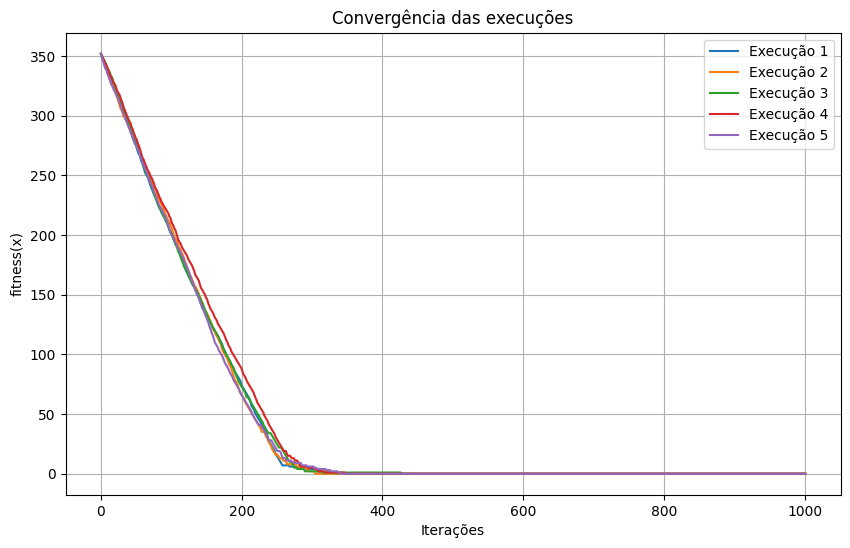
\includegraphics[width=\columnwidth,trim=1 1 1 1,clip]{convergencia_execucoes_p1.png}
    \caption{\label{fig:convergencia_execucoes_p1}Convergência do BVNS implementado para o Problema 1 Isolado.}
\end{figure}

\begin{figure}[htbp]
    \centering
    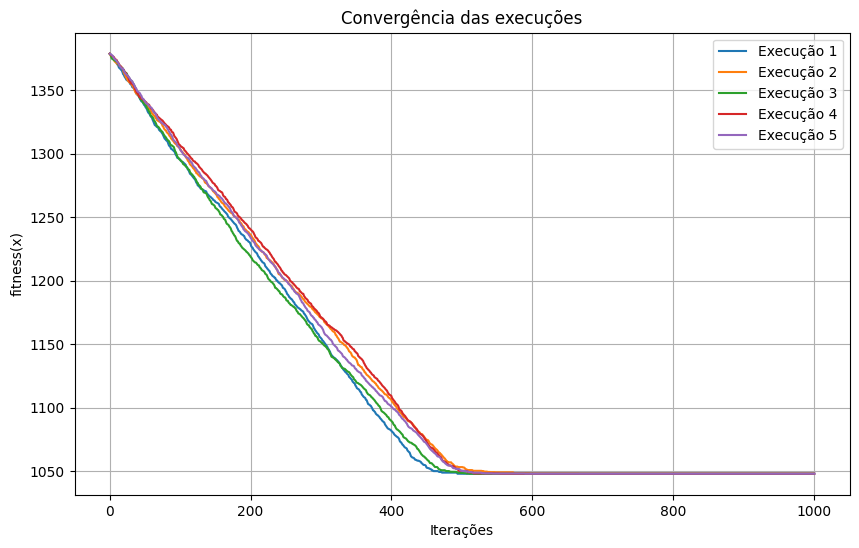
\includegraphics[width=\columnwidth,trim=1 1 1 1,clip]{convergencia_execucoes.png}
    \caption{\label{fig:convergencia_execucoes_p2}Convergência do BVNS implementado para o Problema 2 Isolado.}
\end{figure}

\subsection{Indicador de Hipervolume (HVI)}

Para a realização do cálculo a métrica de HVI foi permitido o uso de mais de 20 soluções pareto na fronteira, de maneira que o valor para a métrica atingisse
os valores indicados para comparação. Dessa forma, foram utilizadas $200$ soluções e a visualização da fronteira pode ser vista na Figura \ref{fig:plotFronteiraParetoERestrito200pontos}.

\begin{figure}[htbp]
    \centering
    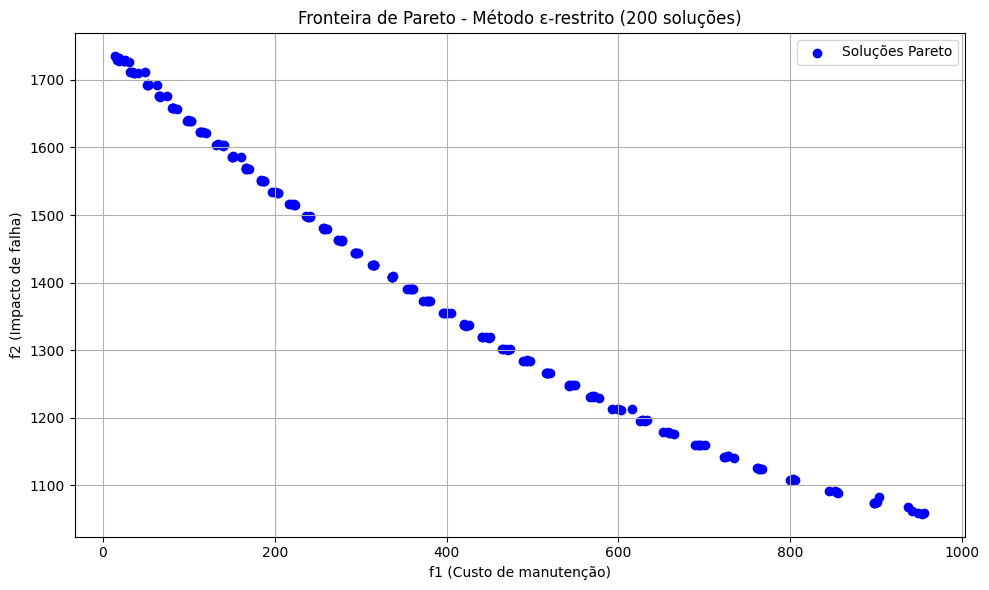
\includegraphics[width=\columnwidth,trim=1 1 1 1,clip]{plotFronteiraParetoERestrito200pontos.png}
    \caption{\label{fig:plotFronteiraParetoERestrito200pontos}Fronteira Pareto para 200 soluções com método $\epsilon$-restrito usada para cálculo do HVI}
\end{figure}

O valor de HVI obtido foi:

\begin{equation}\label{eq:HVI}
	\un{HVI: }0.602974
\end{equation}


\section{Conclusão}
The conclusion goes here.


\begin{thebibliography}{1}

\bibitem{IEEEhowto:kopka}
H.~Kopka and P.~W. Daly, \emph{A Guide to {\LaTeX}}, 3rd~ed.\hskip 1em plus
  0.5em minus 0.4em\relax Harlow, England: Addison-Wesley, 1999.

\end{thebibliography}

\end{document}


